\documentclass[11pt,compress,t,notes=noshow]{beamer}\usepackage[]{graphicx}\usepackage[]{color}

\makeatletter
\def\maxwidth{ %
  \ifdim\Gin@nat@width>\linewidth
    \linewidth
  \else
    \Gin@nat@width
  \fi
}
\makeatother

\definecolor{fgcolor}{rgb}{0.345, 0.345, 0.345}
\newcommand{\hlnum}[1]{\textcolor[rgb]{0.686,0.059,0.569}{#1}}%
\newcommand{\hlstr}[1]{\textcolor[rgb]{0.192,0.494,0.8}{#1}}%
\newcommand{\hlcom}[1]{\textcolor[rgb]{0.678,0.584,0.686}{\textit{#1}}}%
\newcommand{\hlopt}[1]{\textcolor[rgb]{0,0,0}{#1}}%
\newcommand{\hlstd}[1]{\textcolor[rgb]{0.345,0.345,0.345}{#1}}%
\newcommand{\hlkwa}[1]{\textcolor[rgb]{0.161,0.373,0.58}{\textbf{#1}}}%
\newcommand{\hlkwb}[1]{\textcolor[rgb]{0.69,0.353,0.396}{#1}}%
\newcommand{\hlkwc}[1]{\textcolor[rgb]{0.333,0.667,0.333}{#1}}%
\newcommand{\hlkwd}[1]{\textcolor[rgb]{0.737,0.353,0.396}{\textbf{#1}}}%
\let\hlipl\hlkwb

\usepackage{framed}
\makeatletter
\newenvironment{kframe}{%
 \def\at@end@of@kframe{}%
 \ifinner\ifhmode%
  \def\at@end@of@kframe{\end{minipage}}%
  \begin{minipage}{\columnwidth}%
 \fi\fi%
 \def\FrameCommand##1{\hskip\@totalleftmargin \hskip-\fboxsep
 \colorbox{shadecolor}{##1}\hskip-\fboxsep
     \hskip-\linewidth \hskip-\@totalleftmargin \hskip\columnwidth}%
 \MakeFramed {\advance\hsize-\width
   \@totalleftmargin\z@ \linewidth\hsize
   \@setminipage}}%
 {\par\unskip\endMakeFramed%
 \at@end@of@kframe}
\makeatother

\definecolor{shadecolor}{rgb}{.97, .97, .97}
\definecolor{messagecolor}{rgb}{0, 0, 0}
\definecolor{warningcolor}{rgb}{1, 0, 1}
\definecolor{errorcolor}{rgb}{1, 0, 0}
\definecolor{code}{rgb}{0.97, 0.96, 1.0}
\newenvironment{knitrout}{}{} % an empty environment to be redefined in TeX

\usepackage{alltt}
\usepackage[utf8]{inputenc}
\usepackage[ngerman]{babel}
\usepackage{dsfont}
\usepackage{verbatim}
\usepackage{amsmath}
\usepackage{amsfonts}
\usepackage{mathtools}
\usepackage{csquotes}
\usepackage{cmbright}
\usepackage{multirow}
\usepackage{longtable}
\usepackage{enumerate}
\usepackage[absolute,overlay]{textpos}
\usepackage{psfrag}
\usepackage{algorithm}
\usepackage{algpseudocode}
\usepackage{eqnarray}
\usepackage{bytefield}
\usepackage{animate}
\usepackage{tikz}
\usetikzlibrary{shapes,matrix,positioning,chains,arrows,shadows,decorations.pathmorphing,fit,backgrounds}
\usepackage{adjustbox}
\usepackage{colortbl}
\usepackage{tabularx} % for tables (incl. \hline)
\usepackage{arydshln} % Load after array, longtable, colortab and/or colortbl , otherwise problems with \hline in tabular env
\usepackage{etex} %increase registers for \dimenS to more than 256, otherwise we get "No room for a new \dimen"
\usepackage{graphicx}
\usepackage{booktabs} %used in epr lectures
\usepackage{bm} % bold greek letters
\usepackage{hyperref} % url citing
\usepackage{blkarray} % block arrays
\usepackage{listings} % block of code
\usepackage{xcolor} %colored math symbols
\usepackage{pgffor}
\usepackage{verbatimbox}
\usepackage{xcolor}

%some colors
\definecolor{checkgreen}{HTML}{18A126}
\definecolor{errorred}{HTML}{FF0000}
\definecolor{blockbg}{HTML}{F7F7F7}
\definecolor{gray}{HTML}{A0A0A0}

% basic latex stuff
\newcommand{\col}{\par\colorbox{code}{\parbox{\textwidth}{\theverbbox}}\par}
\newcommand{\eg}{e.\,g.\xspace} %for example
\newcommand{\ie}{i.\,e.\xspace} %that is to say...
\newcommand{\pkg}[1]{{\fontseries{b}\selectfont #1}} %fontstyle for R packages
\newcommand{\lz}{\vspace{0.5cm}} %vertical space
\newcommand{\oneliner}[1] % Oneliner for important statements
{\begin{block}{}\begin{center}\begin{Large}#1\end{Large}\end{center}\end{block}}
\def\SpAr{\quad \Rightarrow \quad}

%new environments
\newenvironment{vbframe}  %frame with breaks and verbatim
{
 \begin{frame}[containsverbatim,allowframebreaks]
}
{
\end{frame}
}

\newenvironment{vframe}  %frame with verbatim without breaks (to avoid numbering one slided frames)
{
 \begin{frame}[containsverbatim]
}
{
\end{frame}
}

\newenvironment{blocki}[1]   % itemize block
{
 \begin{block}{#1}\begin{itemize}
}
{
\end{itemize}\end{block}
}

\newenvironment{fragileframe}[2]{  %fragile frame with framebreaks
\begin{frame}[allowframebreaks, fragile, environment = fragileframe]
\frametitle{#1}
#2}
{\end{frame}}

\newcommand{\myframe}[2]{  %short for frame with framebreaks
\begin{frame}[allowframebreaks]
\frametitle{#1}
#2
\end{frame}}

\usepackage{../../style/lmu-lecture}

\let\code=\texttt
\let\proglang=\textsf

\setkeys{Gin}{width=0.9\textwidth}

\usepackage{tikz}
\usetikzlibrary{shapes,arrows,snakes, calc}

% Define block styles
\tikzstyle{decision} = [diamond, draw, text width=6em, text badly centered, node distance=4cm, inner sep=0pt]
\tikzstyle{decision2} = [diamond, draw, fill=customgreen!35, text width=6em, text badly centered, node distance=4cm, inner sep=0pt]

\tikzstyle{block} = [rectangle, draw, text width=14em, text centered, rounded corners, node distance=3cm, minimum height=4em]
\tikzstyle{line} = [draw, -latex']
\tikzstyle{cloud} = [draw, ellipse, node distance=3cm, minimum height=2em]

\title{Introduction to Deep Learning}
\author{Bernd Bischl}
\institute{Department of Statistics -- LMU Munich}
\date{WS 2021/2022}

\setbeamertemplate{frametitle}{\expandafter\uppercase\expandafter\insertframetitle}

\IfFileExists{upquote.sty}{\usepackage{upquote}}{}
\input{../../latex-math/basic-math}
\input{../../latex-math/basic-ml}
\input{../../latex-math/ml-nn}

\title{Deep Learning}

\date{}


\begin{document}
\newcommand{\titlefigure}{plots/frontpage.png}

\newcommand{\learninggoals}{
  \item intution
  \item VAE-parameter fitting
  \item ereparametrization trick
  %\item adversarial training 
}

\lecturechapter{Variational Autoencoder (VAE)}
\lecture{I2DL}


%\newcommand{\vphi}{\bm{\phi}}
%\lecturechapter{10}{Variational Autoencoder (VAE)}
%\lecture{Deeplearning}


\begin{frame}
\frametitle{Variational Autoencoder (VAE): Intution}

%The classic DAG problem: How do we efficiently learn $p_{\thetab}(\mathbf{z}| \xv )$?
    
 Independently proposed by:
\small{
\begin{itemize}
\item Kingma and Welling, \emph{Auto-Encoding Variational Bayes}, ICLR 2014
\item Rezende, Mohamed and Wierstra, \emph{Stochastic back-propagation and variational inference in deep latent Gaussian models.} ICML 2014
\end{itemize}}

\vspace{1mm}

Conventional AEs compute a deterministic feature vector that describes the attributes of the input in latent space:

                \begin{figure}
                \centering
                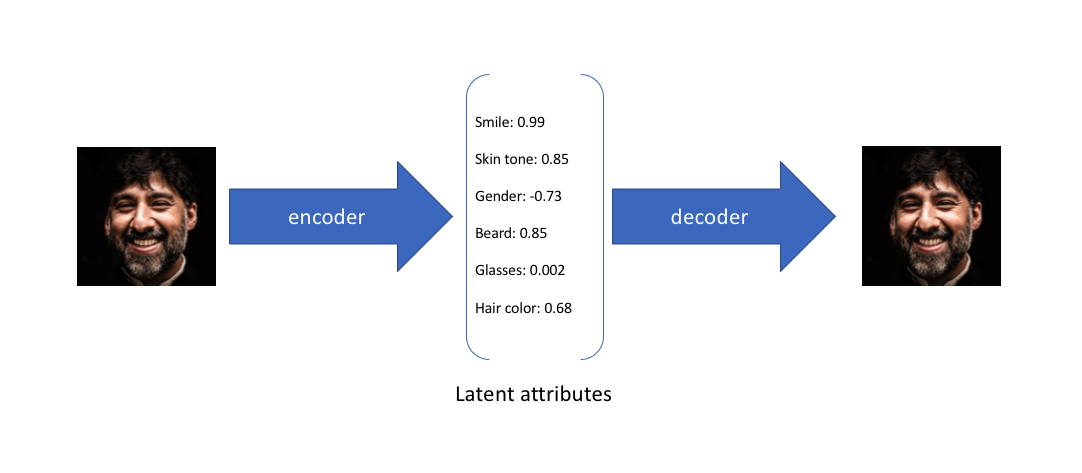
\includegraphics[width=7cm]{plots/ae_intution.png}
                \vspace{-8pt}
                \caption{\tiny{source: https://www.jeremyjordan.me/variational-autoencoders/}}
                \end{figure}
    
\end{frame}

\begin{frame}
\frametitle{Variational Autoencoder (VAE): Intution}

\begin{itemize}
\item Describe each latent attribute as probability distribution
\item Allows to model uncertainty in input data
\end{itemize}

                \begin{figure}
                \centering
                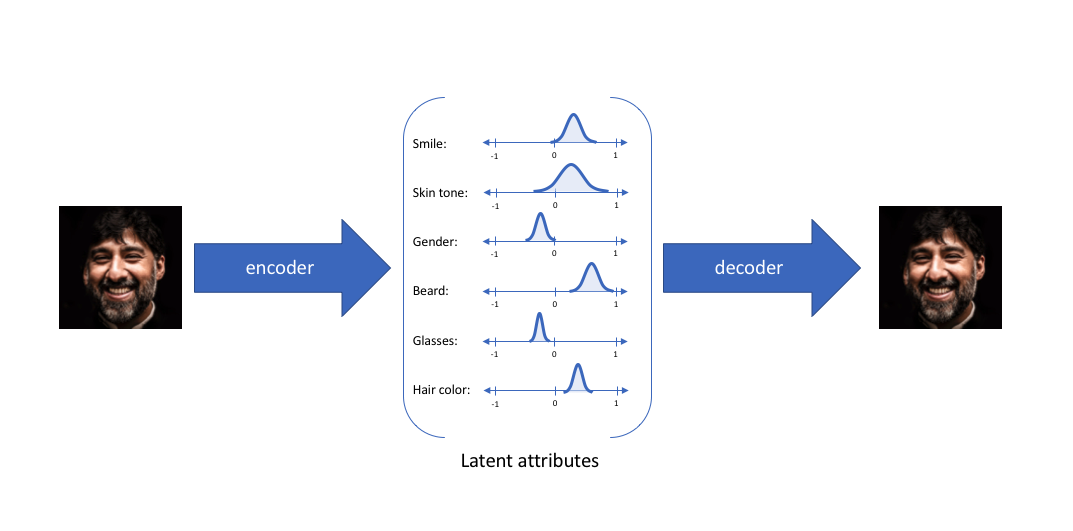
\includegraphics[width=7cm]{plots/vae_intution.png}
                \vspace{-8pt}
                \caption{\tiny{source: https://www.jeremyjordan.me/variational-autoencoders/}}
                \end{figure}
                

\end{frame}



\begin{frame}
\frametitle{Variational Autoencoder (VAE)}

                \begin{figure}
                \centering
                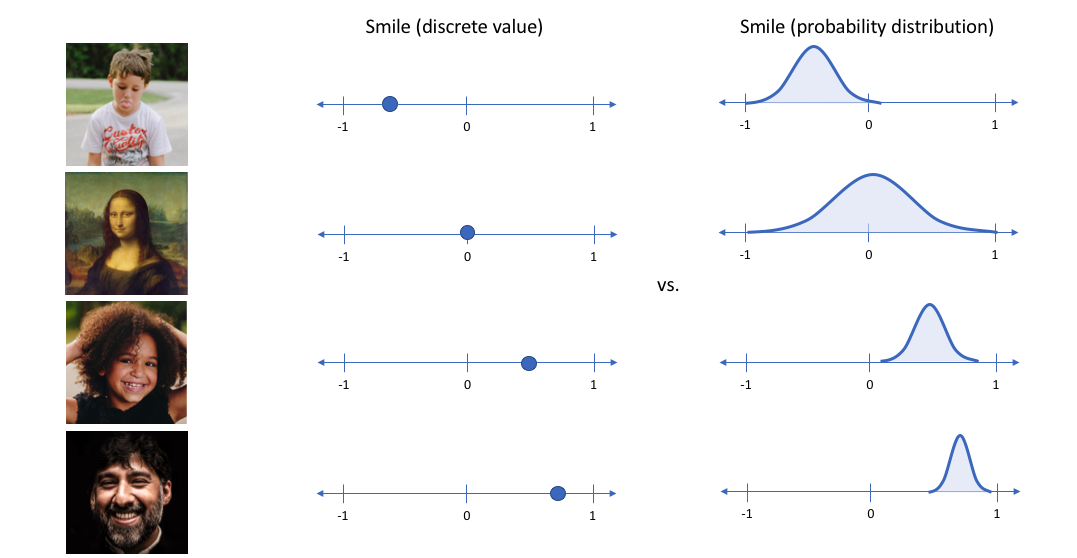
\includegraphics[width=9cm]{plots/vae_motivation.png}
                \vspace{-6pt}
                \caption{\tiny{source: https://www.jeremyjordan.me/variational-autoencoders/}}
                \end{figure}
                \vspace{-10pt}


\begin{itemize}
\item Key difference in variational autoencoders are:
  \begin{itemize}
    \item Uses a variational approach to learn the latent representation
    \item Allows to describe observation in latent space in probablistic manner.
  \end{itemize}     
\end{itemize}  



    
    %Idea: introduce an \textbf{inference model $q_{\vphi }(\mathbf{z}| \xv)$}  that learns to approximate the posterior $p_{\thetab}(\mathbf{z}| \xv )$
    
    %\hspace{1.5cm}\includegraphics[width=0.7\framewidth]{plots/VAE-full.png}




    %Idea: introduce an \textbf{inference model $q_{\vphi }(\mathbf{z}| \xv)$}  that learns to approximate the posterior $p_{\thetab}(\mathbf{z}| \xv )$



%\begin{itemize}
%\item To do inference one would like to calculate $p(\mathbf{z}| \xv ) = \frac{p(\xv| \mathbf{z})p_{\thetab}(\mathbf{z})}{p(\xv)}$.
%
%\pause
%\item But $p_{\thetab}(\xv)=\int p_{\thetab}(\xv|\mathbf{z}) p_{\thetab}(\mathbf{z}) d\mathbf{z}$ is intractable.
%\end{itemize}

%An VAE contains two directed graphical models
%An VAE  consists of directed graphical models

%\vspace{0.7cm}
%\only<1-3>{
    %\hspace{2,3cm}
    %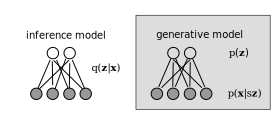
\includegraphics[width=0.7\framewidth]{VAE}
    %\vspace{0.7cm}
    %with distributions
    %with distribution
    %\vspace{-0.4cm}
    %\begin{align}
    % p(\xVec, \hVec)  &= p(\xVec|\hVec_1) p(\hVec_1|\hVec_2) ... p(\hVec_L) \nonumber
    %\end{align}
    %\pause
    %\vspace{-0.4cm}
    %\begin{itemize}
    %\item To do inference one would like to calculate $p(\vec h| \xv ) = \frac{p(\xv| \vec h)p(\vec h)}{p(\xv)}$.
    %
    %\pause
    %\item But $p(\xv)=\int p(\xv|\vec h) p(\vec h) d\vec h$ is intractable.
    %\end{itemize}
    %}
%\only<4>{\hspace{2,3cm} \includegraphics[width=0.7\framewidth]{VAE-full}\\
    
    %with distributions
    %\vspace{-0.4cm}
    %with distribution
    %\begin{align}
    % p(\xVec, \hVec)  &= p(\xVec|\hVec) p(\hVec)  \nonumber \\
    %q(\hVec | \xVec) &= q(\hVec|\xVec) q(\hVec|\hVec_1) ... %q(\hVec_L | \hVec_{L-1}) \nonumber
    % \nonumber
    %\end{align}}

%\small{[Kingma and Welling, Auto-Encoding Variational Bayes, ICLR 2014]}

%\small{[Rezende, Mohamed and Wierstra, Stochastic back-propagation and variational inference in deep latent Gaussian models. ICML 2014]}

\end{frame}


\begin{frame}
\frametitle{VAE: Statistical motivation}

\begin{itemize}
\item Suppose the hidden variable $z$ which generates an observation $x$
\pause
\item By training variational autoencoder, we determin the distribution $z$ and would like to compute $p(z|x)$. \\
\centering{$p\left( {z|x} \right) = \frac{{p\left( {x|z} \right)p\left( z \right)}}{{p\left( x \right)}}$}\\
\vspace{5pt}
\pause
\item \raggedright{However, computing $p(x)$ is difficult since it is an intractable distribution!} \\
\centering{$p\left( x \right) = \int {p\left( {x|z} \right)p\left( z \right)dz}$}\\
\vspace{5pt}
\pause
\item \raggedright{Approximate $p(z|x)$ by tractable distribution $q(z|x)$ which is very similar to $p(z|x)$.} \\

\end{itemize}
\end{frame}

\begin{frame}
\frametitle{VAE: Statistical motivation}

\begin{itemize}
\item \raggedright{KL divergence measures of difference between two probability distributions. Thus, if we wanted to ensure that $q(z|x)$ was similar to $p(z|x)$, we could minimize the KL divergence between the two distributions:} \\
\centering{$\min KL\left( {q\left( {z|x} \right)||p\left( {z|x} \right)} \right)$} \\
\pause
\raggedright{by maximizing the following:}\\
\paused
\centering{$\max {E_{q\left( {z|x} \right)}}\log p\left( {x|z} \right) - KL\left( {q\left( {z|x} \right)||p\left( z \right)} \right)$} \\
\vspace{5pt}
\item \raggedright{The first term represents the reconstruction likelihood and the second term ensures that our learned distribution $q$ is similar to the true prior distribution $p$.}
\item which forces $q(z|x)$ to be similar to true prior distribution $p(z)$

\end{itemize}
\end{frame}


\begin{frame}
\frametitle{VAE: Statistical motivation}

\begin{itemize}
\item $p(z)$ often assumed to be Guassian distribution \\ $\righttarrow$ determining $q(z|x)$ boils down to estimating $\mu$ and $\sigma$.
\item Use neural network to estimate $q(z|x)$ and $p(z|x)$
\end{itemize}


                \begin{figure}
                \centering
                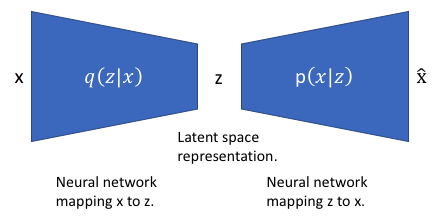
\includegraphics[width=9cm]{plots/vae.png}
                \vspace{-6pt}
                \caption{\tiny{source: https://www.jeremyjordan.me/variational-autoencoders/}}
                \end{figure}
                \vspace{-10pt}

\end{frame}


\begin{frame}
\frametitle{VAE Training}

\end{frame}


\begin{frame}
\frametitle{Reparametrization Trick}

\end{frame}



\begin{frame}
\frametitle{Visualization of latent space}

\end{frame}


\begin{frame}
\frametitle{Variational autoencoders as a generative model}

\end{frame}



\begin{frame}

\begin{itemize}
\item Instead of mapping the input into a fixed vector, we want to map it into a distribution. Let's label this distribution as $p_{\thetab}$, parameterized by ${\thetab}$. The relationship between the data input $x$ and the latent encoding vector $z$ can be fully defined by:

  \begin{itemize}
    \item Prior $p_{\thetab}(\mathbf{z})$
    \item Liklihood $p_{\thetab}( \xv|\mathbf{z})$
    \item Posterior $p_{\thetab}(\mathbf{z} | \xv)$
  \end{itemize}
\end{itemize}

\end{frame}


\begin{frame}
\frametitle{VAE-Parameter Fitting}
\vspace{2mm}

Assuming that we know the real parameter ${\theta}^*$ for this distribution. 

To generate a sample from a real data point $x^{(i)}$:

\begin{itemize}
\item sample $x^{(i)}$ from a prior distribution $p_{{\theta}^*} (z)$
\item a value $x^{(i)}$ is generated from a conditional distribution $p_{{\theta}^*} (x|z=z^{(i)})$ 
\end{itemize}

\vspace{1mm}
The optimal parameter ${\theta}^*$ is the one that maximizes the probability of generating real data samples:

\vspace{2mm}
\centering{
${\theta}^* = \argmax_{\theta} \prod_{i=1}^{n}  p_{\thetab} (x^{(i)})$
}
\vspace{2mm}

we use the log probabilities to convert the product on right-hand side to a sum:

\vspace{2mm}
\centering{
${\theta}^* = \argmax_{\theta} \sum_{i=1}^{n} log p_{\thetab} (x^{(i)})$
}

\end{frame}  

%\end{frame}



\begin{frame}
\frametitle{VAE-Parameter Fitting}
\vspace{2mm}

Now let's update the equation to better demonstrate the data generation process so as to involve the encoding vector:

\vspace{2mm}
\centering{
$ p_{\thetab} (\xv^{(i)}) = \int p_{\thetab} (x^{(i)} | z)  p_{\thetab} (z) dz$ 
}

\vspace{2mm}

Unfortunately it is not easy to compute $ p_{\thetab} (\xv^{(i)}) $ in this way, as it is very expensive to check all the possible values of $z$ and sum them up.
\end{frame}




\begin{frame}
\frametitle{VAE-Parameter Fitting: Variational Lower Bound}

%Since $\log p(\xv_s)$ is intractable, optimization is often based on
%\textbf{variational lower bound} (or \textbf{Evidence Lower BOund (ELBO)})
%\textbf{Evidence Lower BOund (ELBO)}
%of log-likelihood for training example $\xv_s$
    \begin{itemize}
\item $\log p_{\thetab}(\xv)$ is intractable.
\item But we can compute a \textbf{variational lower bound}:
%\textbf{Evidence Lower BOund (ELBO)}
\end{itemize}
%\pause
\only<1>{
    \begin{align*}
    \log p_{\thetab}(\xv) &= \log\int p_{\thetab}(\xv,\mathbf{z}) d\mathbf{z} =  \log \int  q_{\vphi}(\mathbf{z}|\xv) \frac{p_{\thetab}(\xv,\mathbf{z})}{q_{\vphi}(\mathbf{z}|\xv)} d\mathbf{z} \\
    &\color{white}{\geq  \int  q(\vec h|\xv_s)  \log \frac{p(\xv_s,\vec h)}{q(\vec h|\xv_s)} d\vec h }\\
    &\color{white}{\geq \int  q(\vec h|\xv_s)  \big( \log p(\xv_s|\vec h) + \log p(\vec h) - \log q(\vec h|\xv_s) \big)d\vec h} \\
    & \color{white}{mathbb{E}_{q(\vec h|\xv_s)}\big[ \log p(\xv_s|\vec h) \big] - KL\big[ q(\vec h|\xv_s) ||  p(\vec h) \big] }
    \end{align*}}
\only<2>{
    \begin{align*}
    \log p_{\thetab}(\xv) &= \log\int p_{\thetab}(\xv,\mathbf{z}) d\mathbf{z} =  \log \int  q_{\vphi}(\mathbf{z}|\xv) \frac{p_{\thetab}(\xv,\mathbf{z})}{q_{\vphi}(\mathbf{z}|\xv)} d\mathbf{z} \\
    &\color{black}{\geq  \int  q_{\vphi}(\mathbf{z}|\xv)  \log \frac{p_{\thetab}(\xv,\mathbf{z})}{q_{\vphi}(\mathbf{z}|\xv)} d\mathbf{z} }\\
    &\color{white}{= \int  q(\vec h|\xv_s)  \big( \log p(\xv_s|\vec h) + \log p(\vec h) - \log q(\vec h|\xv_s) \big)d\vec h} \\
    & \color{white}{mathbb{E}_{q(\vec h|\xv_s)}\big[ \log p(\xv_s|\vec h) \big] - KL\big[ q(\vec h|\xv_s) ||  p(\vec h) \big] }
    \end{align*}
    \begin{block}{Jensen's inequality}
    Let $f$ be a concave function  and $\mathbf{x}$ an integrable random variable. Then it holds:
        $f(\E{[\mathbf{x}]})  \geq \E{[f(\mathbf{x})]}$.
    \end{block}
    
    
}
\only<3>{
    \begin{align*}
    \log p_{\thetab}(\xv) &= \log\int p_{\thetab}(\xv,\mathbf{z}) d\mathbf{z} =  \log \int  q_{\vphi}(\mathbf{z}|\xv) \frac{p_{\thetab}(\xv,\mathbf{z})}{q_{\vphi}(\mathbf{z}|\xv)} d\mathbf{z} \\
    &\color{black}{\geq  \int  q_{\vphi}(\mathbf{z}|\xv)  \log \frac{p_{\thetab}(\xv,\mathbf{z})}{q_{\vphi}(\mathbf{z}|\xv)} d\mathbf{z} }\\
    %&\color{black}{= \int  q_{\vphi}(\mathbf{z}|\xv)  \big( \log p_{\thetab}(\xv|\mathbf{z}) + \log p_{\thetab}(\mathbf{z}) - \log q_{\vphi}(\mathbf{z}|\xv) \big)d\mathbf{z}} \\
    &\color{black}{= \int  q_{\vphi}(\mathbf{z}|\xv)  \big( \log p_{\thetab}(\xv|\mathbf{z}) + \log \frac{p_{\thetab}(\mathbf{z})}{ q_{\vphi}(\mathbf{z}|\xv)} \big)d\mathbf{z}} \\
    & \color{white}{mathbb{E}_{q(\vec h|\xv_s)}\big[ \log p(\xv_s|\vec h) \big] - KL\big[ q(\vec h|\xv_s) ||  p(\vec h) \big] }
    \end{align*}
    %Todo: Box mit Logarithmus-Regeln einbauen!
}
\only<4>{
    \begin{align*}
    \log p_{\thetab}(\xv) &= \log\int p_{\thetab}(\xv,\mathbf{z}) d\mathbf{z} =  \log \int  q_{\vphi}(\mathbf{z}|\xv) \frac{p_{\thetab}(\xv,\mathbf{z})}{q_{\vphi}(\mathbf{z}|\xv)} d\mathbf{z} \\
    &\color{black}{\geq  \int  q_{\vphi}(\mathbf{z}|\xv)  \log \frac{p_{\thetab}(\xv,\mathbf{z})}{q_{\vphi}(\mathbf{z}|\xv)} d\mathbf{z} }\\
    &\color{black}{= \int  q_{\vphi}(\mathbf{z}|\xv)  \big( \log p_{\thetab}(\xv|\mathbf{z}) + \log \frac{p_{\thetab}(\mathbf{z})}{ q_{\vphi}(\mathbf{z}|\xv)} \big)d\mathbf{z}} \\
    & \color{black}{=\mathbb{E}_{q_{\vphi}(\mathbf{z}|\xv)}\big[ \log p_{\thetab}(\xv|\mathbf{z}) \big] - KL\big[ q_{\vphi}(\mathbf{z}|\xv) ||  p_{\thetab}(\mathbf{z}) \big] }
    \end{align*}}
\only<5>{
    \begin{align*}
    \log p_{\thetab}(\xv) &= \log\int p_{\thetab}(\xv,\mathbf{z}) d\mathbf{z} =  \log \int  q_{\vphi}(\mathbf{z}|\xv) \frac{p_{\thetab}(\xv,\mathbf{z})}{q_{\vphi}(\mathbf{z}|\xv)} d\mathbf{z} \\
    &\color{black}{\geq  \int  q_{\vphi}(\mathbf{z}|\xv)  \log \frac{p_{\thetab}(\xv,\mathbf{z})}{q_{\vphi}(\mathbf{z}|\xv)} d\mathbf{z} }\\
    &\color{black}{= \int  q_{\vphi}(\mathbf{z}|\xv)  \big( \log p_{\thetab}(\xv|\mathbf{z}) + \log \frac{p_{\thetab}(\mathbf{z})}{ q_{\vphi}(\mathbf{z}|\xv)} \big)d\mathbf{z}} \\
    & \color{black}{=\underbrace{\mathbb{E}_{q_{\vphi}(\mathbf{z}|\xv)}\big[ \log p_{\thetab}(\xv|\mathbf{z}) \big] - KL\big[ q_{\vphi}(\mathbf{z}|\xv) ||  p_{\thetab}(\mathbf{z}) \big] }_{:=ELBO(\thetab, \vphi, \xv)} }
    \end{align*}}

\end{frame}


\begin{frame}
\frametitle{VAE-Parameter Fitting: Variational Lower Bound}

\only<1>{
    \begin{equation*}
    ELBO(\thetab, \vphi, \xv) = \mathbb{E}_{q_{\vphi}(\mathbf{z}|\xv)}\big[ \log p_{\thetab}(\xv|\mathbf{z}) \big] - KL\big[ q_{\vphi}(\mathbf{z}|\xv) ||  p_{\thetab}(\mathbf{z}) \big]
    \end{equation*}
    %\begin{itemize}
    %\item \color{white}{First term resembles reconstruction loss}
    %\item \color{white}{Second  term penalizes encoder for deviating from prior}
    %\end{itemize}
}
\only<2>{
    \begin{equation*}
    ELBO(\thetab, \vphi, \xv) = \mathbb{E}_{q_{\vphi}(\mathbf{z}|\xv)}\big[ \log p_{\thetab}(\xv|\mathbf{z}) \big] - KL\big[ q_{\vphi}(\mathbf{z}|\xv) ||  p_{\thetab}(\mathbf{z}) \big]
    \end{equation*}
    \begin{itemize}
    \item Also known as \textbf{Evidence Lower BOund (ELBO)}.
    %\item \color{black}{First term resembles reconstruction loss}
    %\item \color{white}{Second  term penalizes encoder for deviating from prior}
    \end{itemize}
}
\only<3>{
    \begin{equation*}
    ELBO(\thetab, \vphi, \xv) = \color{red}{\mathbb{E}_{q_{\vphi}(\mathbf{z}|\xv)}\big[ \log p_{\thetab}(\xv|\mathbf{z}) \big]} \color{black}{- KL\big[ q_{\vphi}(\mathbf{z}|\xv) ||  p_{\thetab}(\mathbf{z}) \big]}
    \end{equation*}
    \begin{itemize}
    \item Also known as \textbf{Evidence Lower BOund (ELBO)}.
    \item \color{black}{First term resembles reconstruction loss}.
    %\item \color{white}{Second  term penalizes encoder for deviating from prior}
    \end{itemize}
}
\only<4>{
    \begin{equation*}
    ELBO(\thetab, \vphi, \xv) = \color{black}{\mathbb{E}_{q_{\vphi}(\mathbf{z}|\xv)}\big[ \log p_{\thetab}(\xv|\mathbf{z}) \big]} \color{red}{- KL\big[ q_{\vphi}(\mathbf{z}|\xv) ||  p_{\thetab}(\mathbf{z}) \big]}
    \end{equation*}
    \begin{itemize}
    \item Also known as \textbf{Evidence Lower BOund (ELBO)}.
    \item \color{black}{First term resembles reconstruction loss}.
    \item \color{black}{Second  term penalizes encoder for deviating from prior}.
    \end{itemize}
}
\only<5>{
    \begin{equation*}
    ELBO(\thetab, \vphi, \xv) = \mathbb{E}_{q_{\vphi}(\mathbf{z}|\xv)}\big[ \log p_{\thetab}(\xv|\mathbf{z}) \big] - KL\big[ q_{\vphi}(\mathbf{z}|\xv) ||  p_{\thetab}(\mathbf{z}) \big]
    \end{equation*}
    \begin{itemize}
    \item Also known as \textbf{Evidence Lower BOund (ELBO)}.
    \item \color{black}{First term resembles reconstruction loss.}
    \color{black}{ \item Second  term penalizes encoder for deviating from prior.}
    \item It can be shown that
    %$\log p(\xv_s) = ELBO(q(\vec h|\xv_s)) + KL\big[ q(\vec h|\xv_s) ||  p(\vec h|\xv ) \big]$
        $ELBO(\thetab, \vphi, \xv) = \log p_{\thetab}(\xv) -  KL\big[ q_{\vphi}(\mathbf{z}|\xv) ||  p_{\thetab}(\mathbf{z}|\xv ) \big]$\\
    $\Rightarrow$ by maximizing the ELBO we maximize $p_{\thetab}(\xv)$ and minimize $KL\big[ q_{\vphi}(\mathbf{z}|\xv) ||  p_{\thetab}(\mathbf{z}|\xv ) \big]$.
    \end{itemize}
}


\end{frame}


\frame{
    \frametitle{VAE-Model Definition}
    
    %Idea: Use a NN to learn a mapping from some latent variable $\mathbf{z}$ to a complicated distribution on $\xv$.
    
    %$$p(\xv) = \int p(\xv, \mathbf{z}) d\mathbf{z} = \int p(\xv| \vec %z) p_{\thetab}(\mathbf{z}) d\mathbf{z}$$
            %where $p_{\thetab}(\mathbf{z})$ is a some simple distribution and $ p(\xv| \mathbf{z})=g(\mathbf{z})$
            %$$p(\xv, \mathbf{z}) = p(\xv| \mathbf{z}) p_{\thetab}(\mathbf{z})$$
            
            Idea:
            \begin{itemize}
        \item Set $p_{\thetab}(\mathbf{z})$ to some simple distribution. % e.g. $\mathcal{N}(1,0)$.
        \item Parametrize inference model and generative model with  neural networks $f(\xv, \vphi)$ and $g(\mathbf{z}, \thetab)$.
        \end{itemize}
        
        
        \begin{figure}
        \centering
        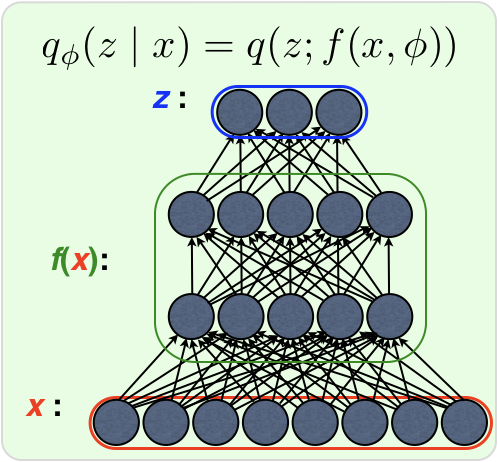
\includegraphics[width=5cm]{plots/VAE-inferenceModel.png}
        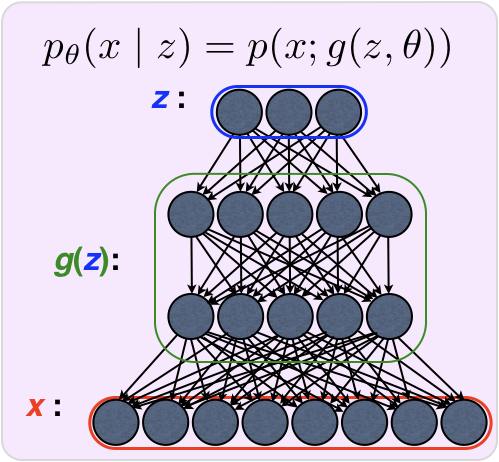
\includegraphics[width=5cm]{plots/VAE-generativeModel2.png}
        \end{figure}
        
}

\frame{
    \frametitle{VAE-Model Definition}
    
    %Idea: Use a NN to learn a mapping from some latent variable $\mathbf{z}$ to a complicated distribution on $\xv$.
    
    %$$p(\xv) = \int p(\xv, \mathbf{z}) d\mathbf{z} = \int p(\xv| \vec %z) p_{\thetab}(\mathbf{z}) d\mathbf{z}$$
            %where $p_{\thetab}(\mathbf{z})$ is a some simple distribution and $ p(\xv| \mathbf{z})=g(\mathbf{z})$
            %$$p(\xv, \mathbf{z}) = p(\xv| \mathbf{z}) p_{\thetab}(\mathbf{z})$$
            
            
            \only<1>{
                %\vspace{-0.8cm}
                Usually:
                    \begin{itemize}
                \item $f(\xv, \vphi)= \left( \bm{\mu}_{\mathbf{z}}(\xv), \bm{\sigma}_{\mathbf{z}}(\xv) \right)$ and $q_{\vphi}(\mathbf{z}| \xv) = \mathcal{N}(\mathbf{z}; \bm{\mu}_{\mathbf{z}}(\xv), \bm{\sigma}^2_{\mathbf{z}}(\xv))$
                    %\item \color{white}{$p_{\thetab}(\mathbf{z})= \mathcal{N}(\mathbf{z}; 1,0)$}
                %\item \color{white}{$g(\mathbf{z})= \left( \mu_{\xv}(\mathbf{z}), \sigma_{\xv}(\mathbf{z}) \right)$ and $p_{\thetab}(\mathbf{z}| \xv) = \mathcal{N}(\mathbf{z}; \bm{\mu}_{\xv}(\mathbf{z}), \bm{\sigma}_{\xv}(\mathbf{z}))$}
                \end{itemize}
                
                \vspace{1.3cm}
                \begin{figure}
                \hspace{-6cm}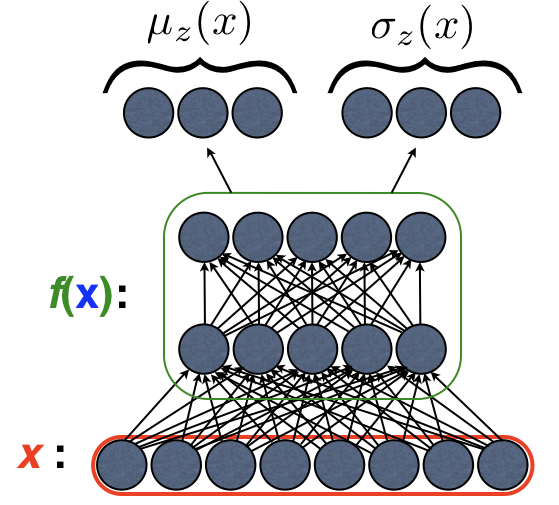
\includegraphics[width=5cm]{plots/VAE-inferenceModelGaussian.png}
                %\includegraphics[width=6cm]{VAE-generativeModelGaussian.png}
                \end{figure}
            }
        
        \only<2>{
            Usually:
                \begin{itemize}
            \item $f(\xv, \vphi)= \left( \bm{\mu}_{\mathbf{z}}(\xv), \bm{\sigma}_{\mathbf{z}}(\xv) \right)$ and $q_{\vphi}(\mathbf{z}| \xv) = \mathcal{N}(\mathbf{z}; \bm{\mu}_{\mathbf{z}}(\xv), \bm{\sigma}^2_{\mathbf{z}}(\xv))$
                \item $p_{\thetab}(\mathbf{z})= \mathcal{N}(\mathbf{z}; 0,1)$
                    \pause
                \item $g(\mathbf{z}, \thetab)= \left( \bm{\mu}_{\xv}(\mathbf{z}), \bm{\sigma}_{\xv}(\mathbf{z}) \right)$ and $p_{\thetab}(\xv| \mathbf{z}) = \mathcal{N}(\xv; \bm{\mu}_{\xv}(\mathbf{z}), \bm{\sigma}^2_{\xv}(\mathbf{z}))$
                    \end{itemize}
                
                
                \begin{figure}
                \centering
                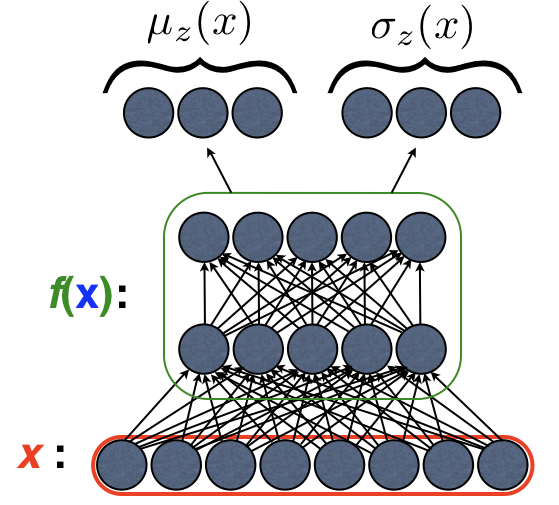
\includegraphics[width=5cm]{plots/VAE-inferenceModelGaussian.png}
                \includegraphics[width=6cm]{plots/VAE-generativeModelGaussian.png}
                \end{figure}
        }
        
}





\begin{frame}
\frametitle{VAE-Parameter Fitting: reparameterization Trick}
\begin{itemize}
\item Goal: Learn parameters $\vphi$ and $\thetab$ by maximizing %the ELBO (lower bound of $\log p_{\thetab}(\xv)$) by gradient ascent.
\begin{equation*}
ELBO(\thetab, \vphi, \xv) = \mathbb{E}_{q_{\vphi}(\mathbf{z}|\xv)}\big[ \log p_{\thetab}(\xv|\mathbf{z}) \big] - KL\big[ q_{\vphi}(\mathbf{z}|\xv) ||  p_{\thetab}(\mathbf{z}) \big]
\end{equation*}
based on gradient ascent.
\item Idea: Approximate first term
\begin{align*}
\mathbb{E}_{q_{\vphi}(\mathbf{z}|\xv)}\big[ \log p_{\thetab}(\xv|\mathbf{z}) \big] &= \mathbb{E}_{\mathbf{z} \sim \mathcal{N}(\mathbf{z}; \bm{\mu}_{\mathbf{z}}(\xv), \bm{\sigma}_{\mathbf{z}}(\xv))}\big[ \log p_{\thetab}(\xv|\mathbf{z}) \big]\\
&\approx \frac{1}{L} \sum_{l=1}^{L} \log p_{\thetab}(\xv|\mathbf{z}^{(l)})
\end{align*}
\item  Problem:
    %Given $\mathbf{z} \sim q_{\vphi}(\mathbf{z}| \xv)$,
Given this average,
how should one take derivatives
%(a function of) $\mathbf{z}$
    %$ q_{\vphi}(\mathbf{z}| \xv)$
    w.r.t.~$\vphi$?
    %\item Solution:
    % For $ q_{\vphi}(\vec h| \xv) =\mathcal{N}(\bm{\mu}, \bm{\sigma})$, $\vphi=(\bm{\mu}, \bm{\sigma})$ \\ reparametrize: $\alert{\vec h= \bm{\mu} + \bm{\sigma} \odot \bm{\epsilon}}$, with $\alert{\bm{\epsilon} \sim \mathcal{N}(\mathbf{0}, \mathbf{1})}$
    %\item and let $(\bm{\mu}, \bm{\sigma})=f(\xv)$ be a function given by a neural network.
\end{itemize}

\end{frame}


\begin{frame}
\frametitle{VAE-Parameter Fitting: reparameterization Trick}

\begin{block}{Recall: Linear transformation of a normal random variable}
\begin{center}
Let $\bm{\epsilon}$ be standard normally distributed, i.e. $\bm{\epsilon} \sim\mathcal{N}(\bm{\epsilon}; \mathbf{0}, \mathbf{1})$. Then for $\mathbf{z} = \bm{\epsilon} \cdot \bm{\sigma} + \bm{\mu} $ it holds: $\mathbf{z}\sim \mathcal{N}(\mathbf{z}; \bm{\mu}, \bm{\sigma}^2)$
    \end{center}
\end{block}
\only<2>{
    Back to our problem:
        \begin{align*}
    \mathbb{E}_{q_{\vphi}(\mathbf{z}|\xv)}\big[ \log p_{\thetab}(\xv|\mathbf{z}) \big] &= \mathbb{E}_{\mathbf{z} \sim \mathcal{N}(\mathbf{z}; \bm{\mu}_{\mathbf{z}}(\xv), \bm{\sigma}_{\mathbf{z}}(\xv))}\big[ \log p_{\thetab}(\xv|\mathbf{z}) \big]\\
    &\approx \frac{1}{L} \sum_{l=1}^{L} \log p_{\thetab}(\xv|\mathbf{z}^{(l)})
    \end{align*}
    Solution: Define \color{red}{$\mathbf{z} = \bm{\epsilon} \cdot \bm{\sigma}_{\mathbf{z}}(\xv )+ \bm{\mu}_{\mathbf{z}}(\xv ) $} \color{black}{ where} \color{red}{$\bm{\epsilon} \sim\mathcal{N}(\bm{\epsilon}; \mathbf{0}, \mathbf{1})$. }
}
\only<3>{
    Back to our problem:
        \begin{align*}
    \mathbb{E}_{q_{\vphi}(\mathbf{z}|\xv)}\big[ \log p_{\thetab}(\xv|\mathbf{z}) \big] &= \mathbb{E}_{\color{red}{\bm{\epsilon} \sim\mathcal{N}(\bm{\epsilon}; \mathbf{0}, \mathbf{1})}}\big[ \log p_{\thetab}(\xv|\mathbf{z}) \big]\\
    &\approx \frac{1}{L} \sum_{l=1}^{L} \log p_{\thetab}(\xv|\mathbf{z}^{(l)})
    \end{align*}
    Solution: Define \color{red}{$\mathbf{z} = \bm{\epsilon} \cdot \bm{\sigma}_{\mathbf{z}}(\xv )+ \bm{\mu}_{\mathbf{z}}(\xv ) $} \color{black}{ where} \color{red}{$\bm{\epsilon} \sim\mathcal{N}(\bm{\epsilon}; \mathbf{0}, \mathbf{1})$. }
}
\only<4>{
    Back to our problem:
        \begin{align*}
    \mathbb{E}_{q_{\vphi}(\mathbf{z}|\xv)}\big[ \log p_{\thetab}(\xv|\mathbf{z}) \big] &= \mathbb{E}_{\color{red}{\bm{\epsilon} \sim\mathcal{N}(\bm{\epsilon}; \mathbf{0}, \mathbf{1})}}\big[ \log p_{\thetab}(\xv|\color{red}{\mathbf{z} = \bm{\epsilon} \cdot \bm{\sigma}_{\mathbf{z}}(\xv )+ \bm{\mu}_{\mathbf{z}}(\xv ) }\color{black}{) \big]}\\
        &\approx \frac{1}{L} \sum_{l=1}^{L} \log p_{\thetab}(\xv|\mathbf{z}^{(l)})
        \end{align*}
        Solution: Define \color{red}{$\mathbf{z} = \bm{\epsilon} \cdot \bm{\sigma}_{\mathbf{z}}(\xv )+ \bm{\mu}_{\mathbf{z}}(\xv ) $}\color{black}{ where} \color{red}{$\bm{\epsilon} \sim\mathcal{N}(\bm{\epsilon}; \mathbf{0}, \mathbf{1})$. }
}
\only<5>{
    Back to our problem:
        \begin{align*}
    \mathbb{E}_{q_{\vphi}(\mathbf{z}|\xv)}\big[ \log p_{\thetab}(\xv|\mathbf{z}) \big] &= \mathbb{E}_{\color{red}{\bm{\epsilon} \sim\mathcal{N}(\bm{\epsilon}; \mathbf{0}, \mathbf{1})}}\big[ \log p_{\thetab}(\xv|\color{red}{\mathbf{z} = \bm{\epsilon} \cdot \bm{\sigma}_{\mathbf{z}}(\xv )+ \bm{\mu}_{\mathbf{z}}(\xv ) }\color{black}{) \big]}\\
        &\approx \frac{1}{L} \sum_{l=1}^{L} \log p_{\thetab}(\xv|\color{red}{\mathbf{z}^{(l)} = \bm{\epsilon}^{(l)} \cdot \bm{\sigma}_{\mathbf{z}}(\xv )+ \bm{\mu}_{\mathbf{z}}(\xv ) } )
        \end{align*}
        Solution: Define \color{red}{$\mathbf{z} = \bm{\epsilon} \cdot \bm{\sigma}_{\mathbf{z}}(\xv )+ \bm{\mu}_{\mathbf{z}}(\xv ) $}\color{black}{ where} \color{red}{$\bm{\epsilon} \sim\mathcal{N}(\bm{\epsilon}; \mathbf{0}, \mathbf{1})$. }
}

\end{frame}



\frame{
    \frametitle{VAE-Training with Backpropagation}
    
    Due to the reparameterization trick, we can simultaneously train both the generative model  $p_{\thetab}(\xv| \mathbf{z})$  and the inference model $q_{\vphi}(\mathbf{z}| \xv)$   by maximizing the ELBO based on gradient ascent and backpropagation.
    
    
    
    \begin{figure}
    \centering
    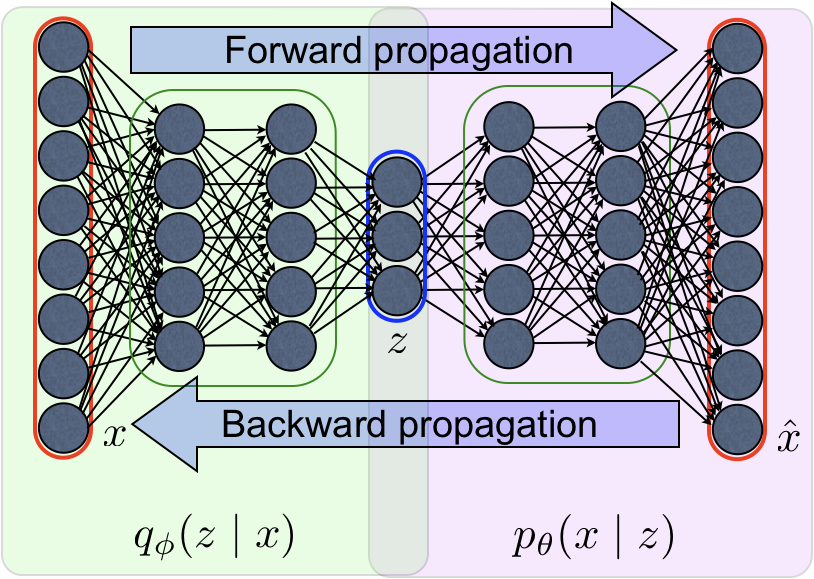
\includegraphics[width=6cm]{plots/VAE-BackProp.png}
    \end{figure}
    
}

\begin{frame}{Illustration of forward pass}
  \begin{figure}
    \centering
    \scalebox{1}{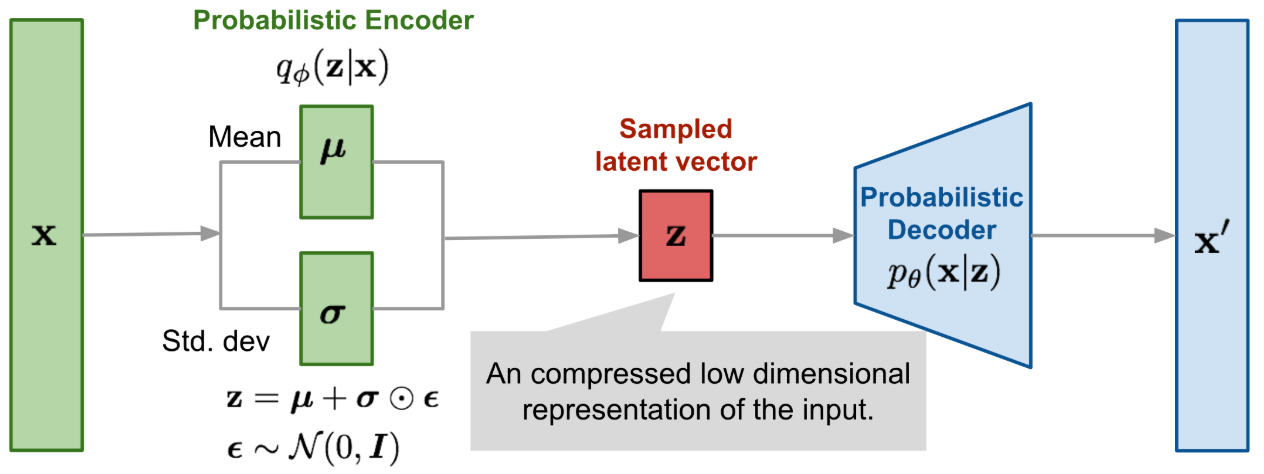
\includegraphics{plots/vae_forwardpass.png}}
    \tiny{\\ credit: Lillian Weng}
    \caption{\footnotesize Illustration of the forward pass in a VAE. For a given $\xv$, the encoder network outputs the mean(s) $\bm{\mu}_{\mathbf{z}}(\xv)$ and standard deviation(s) $\bm{\sigma}_{\mathbf{z}}(\xv)$ of $\mathcal{N}(\mathbf{z}; \bm{\mu}_{\mathbf{z}}(\xv), \bm{\sigma}^2_{\mathbf{z}}(\xv))$. From this, a vector $\mathbf{z}$ is sampled and fed to the decoder network which gives us $\xv'$. If $\xv$ is an image, $\xv'$ is commonly interpreted as the reconstructed image. }
    \end{figure}
\end{frame}

\frame{
    \frametitle{Latent Variables learned by a VAE}
    
    \begin{figure}
    \centering
    \scalebox{0.4}{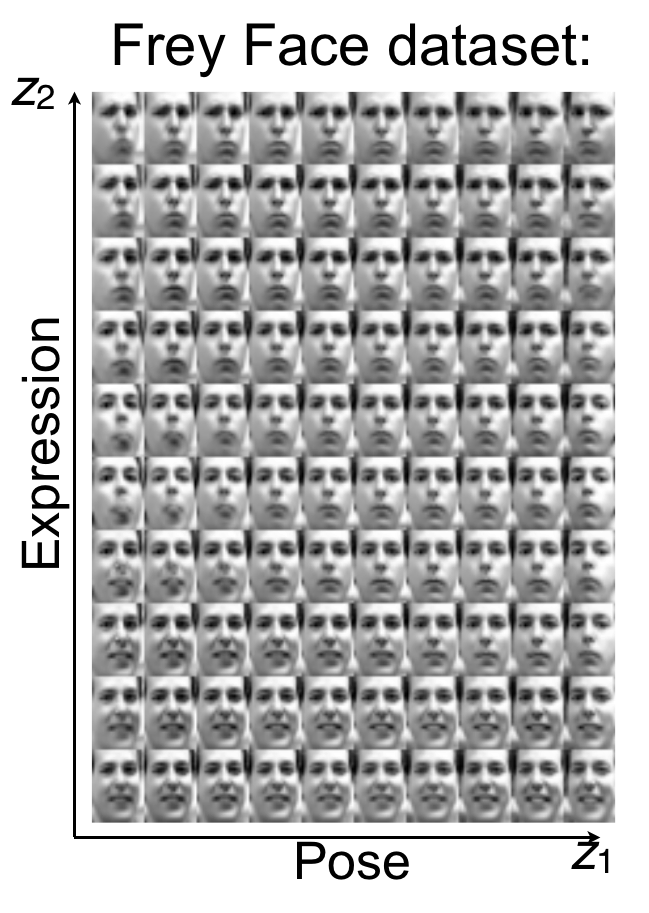
\includegraphics{plots/LatentVariables-FF.png}}
    \caption{\footnotesize Images generated by a VAE are superimposed on the latent vectors that generated them. In the two-dimensional latent space of the VAE, the first dimension encodes the position of the face and the second dimension encodes the expression. Therefore, starting at any point in the latent space, if we move along either axis, the corresponding property will change in the generated image.    (Goodfellow et al.,  2016)}
    \end{figure}
    
}

\frame{
    \frametitle{Latent Variables learned by a VAE}
    
    \begin{figure}
    \centering
    \scalebox{0.5}{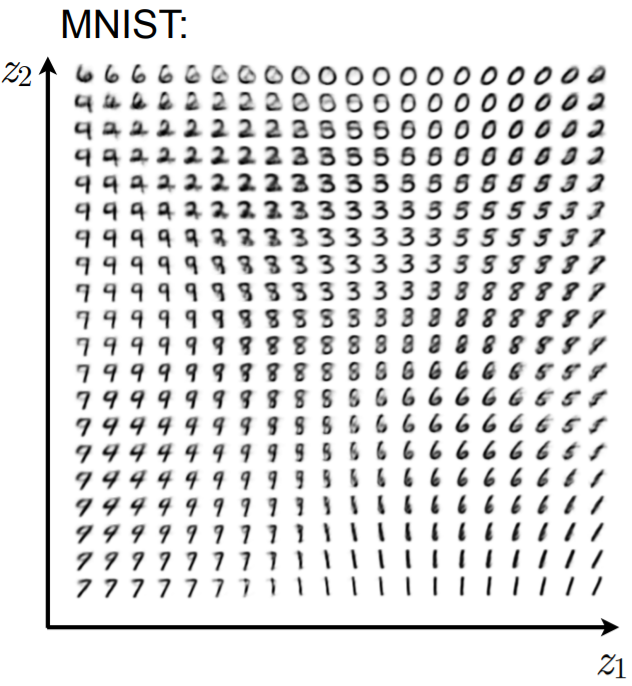
\includegraphics{plots/vae_mnist_n.png}}
    \caption{\footnotesize Images generated by a VAE are superimposed on the latent vectors that generated them. The two-dimensional latent space of the VAE captures much of the variation present in MNIST. Different regions in the latent space correspond to different digits in the generated images. (Goodfellow et al.,  2016)}
    \end{figure}
    
}



\frame{
    \frametitle{Samples from a vanilla VAE}
    
    % \begin{figure}
    % \centering
    % 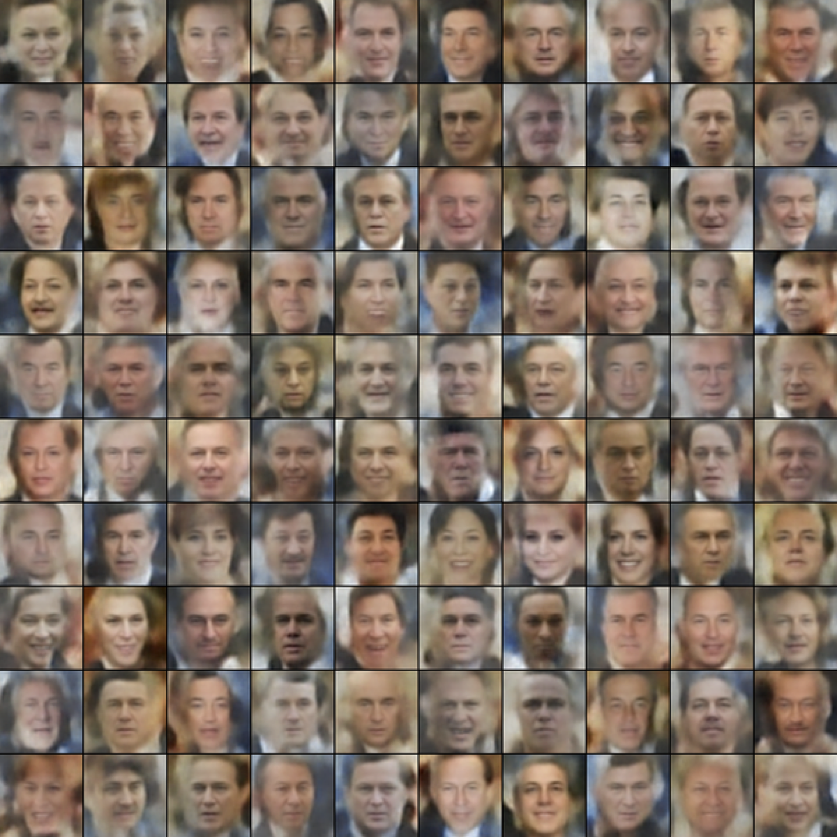
\includegraphics[width=5cm]{plots/SamplesVAE-Faces.png}
    % %\hspace{0.3cm}
    % 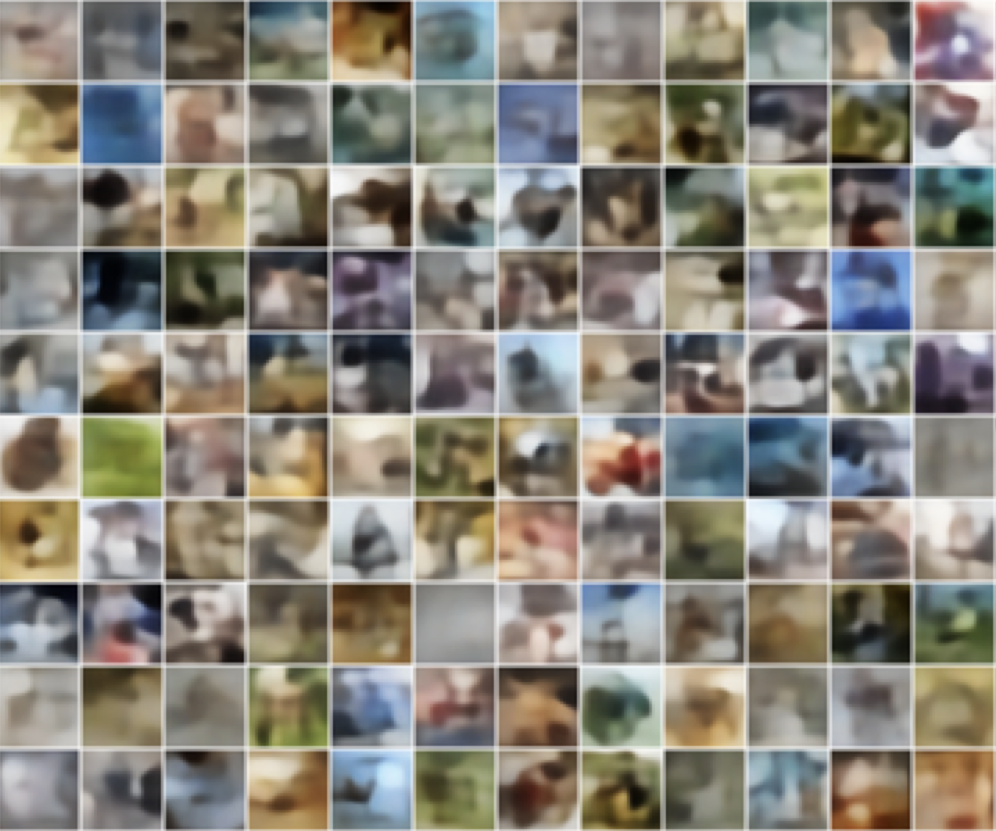
\includegraphics[width=6cm]{plots/SamplesVAE-ImageNet.png}
    % \caption{\footnotesize Samples generated by a VAE trained on }
    % \end{figure}
    % %\vspace{-1cm}
    % \texttt{ \small{ Labeled Faces in the Wild (LFW)}    \;\;\;\;\;\;\;\;\;\;\;\ \small{ImageNet (small)}}
    % %
    
    \begin{figure}
      \centering
      \scalebox{0.9}{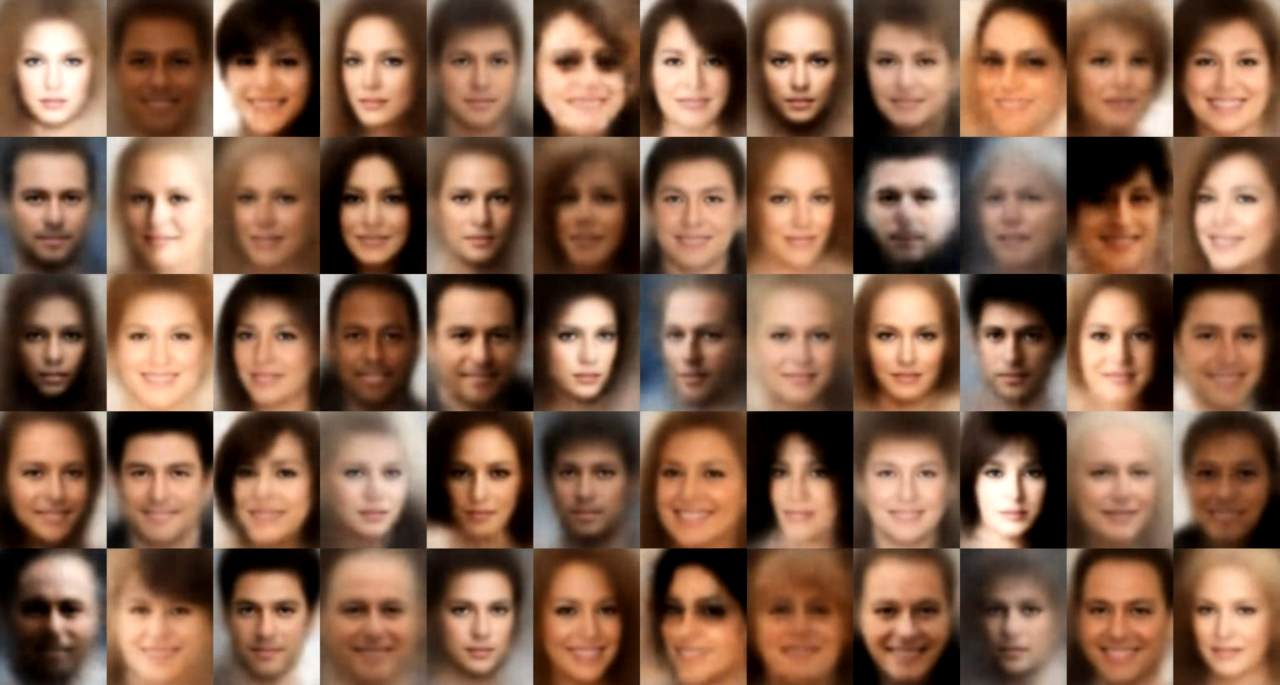
\includegraphics{plots/vae_faces.png}}
      \tiny{\\ Credit : Wojciech Mormul}
      \caption{\footnotesize Samples generated by a VAE that was trained on images of people's faces.}
    \end{figure}
}




%%%%%%%%%%%%%%%%%%%%%%%%%%%%%%%%%%%%%%%%%%%%%%%%%%%%%%%%%%%%%%%%%%
%%%%%%%%%%%%%%%%%%          REFERENCES          %%%%%%%%%%%%%%%%%%
%%%%%%%%%%%%%%%%%%%%%%%%%%%%%%%%%%%%%%%%%%%%%%%%%%%%%%%%%%%%%%%%%%
\begin{vbframe}
\frametitle{References}
\footnotesize{
\begin{thebibliography}{99}
%%%%%%%%%%%%%%%%%%%%%%%%%%%%%%%%%%
\bibitem[Weng, 2014]{5} Lilian Weng (2018)
\newblock From Autoencoder to Beta-VAE
\newblock \emph{\url{https://lilianweng.github.io/lil-log/2018/08/12/from-autoencoder-to-beta-vae.html}}
%%%%%%%%%%%%%%%%%%%%%%%%%%%%%%%%%%
%%%%%%%%%%%%%%%%%%%%%%%%%%%%%%%%%

\end{thebibliography}
}
\end{vbframe}
%%%%%%%%%%%%%%%%%%%%%%%%%%%%%%%%%%%%%%%%%%%%%%%%%%%%%%%%%%%%%%%%%%
%%%%%%%%%%%%%%%%%%%%%%%%%%%%%%%%%%%%%%%%%%%%%%%%%%%%%%%%%%%%%%%%%%

\endlecture
\end{document}

